\documentclass[a4paper,14pts]{report}
\usepackage{settings-my-thesis}
\includeonly{ introduzione/intro,%
               capitoli/capitolo-1,%
               capitoli/capitolo-2,%
               capitoli/capitolo-3,%
              }
\begin{document}
\titlepage{

\includegraphics[keepaspectratio]{logoSapienza}
\\
\vspace{150pt}
\begin{center}
{\onehalfspacing
\huge{\textcolor{Mahogany!80!BrickRed}{\textsf{Uno Schema Semi-Lagrangiano per il Moto per Curvatura Media che preserva il Volume}}}}
\end{center}
\vspace{150pt}
{\small\textcolor{Mahogany!80!BrickRed}{\textsf{Facoltà di Scienze Matematiche Fisiche e Naturali}\\
\textsf{Corso di Laurea Magistrale in Matematica per le Applicazioni}}\\
\textsf{Michele Cipolla\\
n° matricola 1174687}\vspace{50pt}
\\
\textsf{Relatrice:\\
Prof.Elisabetta Carlini}\\
\\
\bigskip
\textsf{Anno Accademico 2013/2014}
}}

\cleardoublepage
\pdfbookmark{\contentsname}{Contents}
\tableofcontents
\listoffigures
\chapter*{INTRODUZIONE}
\phantomsection
\addcontentsline{toc}{chapter}{Introduzione}
WORKING IN PROGRESS \cite[vedi][]{vpmcm:code}.

\chapter{Evoluzione Geometrica Per Curvatura Media}
'WIP'
%%%%%%%%%%%%%%%%%%%%%%%%%%%%%%%%%%%%%%%%%%%%%%%%%%%%
%
% Section 1.1
%
%%%%%%%%%%%%%%%%%%%%%%%%%%%%%%%%%%%%%%%%%%%%%%%%%%%%
\section{Qualcosa sulle Superfici in $\mathbb{R}^3$}

Consideriamo un sottoinsieme $S\subseteq\mathbb{R}^3$, diremo che è una superficie regolare se per ogni punto $p\in S$ esiste un intorno $V$ di $p$ in $\mathbb{R}^3$, un aperto $U\subset\mathbb{R}^2$ e un'applicazione differenziabile $\mathcal{S}:U\longrightarrow V\cap S$ tale che:
\begin{enumerate}
  \item $\mathcal{S}$ è un omeomorfismo,
  \item il differenziale $d\mathcal{S}$ ha rango massimo in ogni punto di $U$.
\end{enumerate}
L'applicazione $\mathcal{S}$ si dice parametrizzazione regolare in un intorno del punto $p$. Mentre l'insieme $V\cap S=\mathcal{S}(U)$ si dice porzione di superficie parametrica regolare. La condizione di regolarità, ci esclude superfici che intersecano se stesse.

Siano $u$ e $v$ coordinate su $U\subset\mathbb{R}^2$ , $S = \mathcal{S}(U)$ e $p=\mathcal{S}(u_0,v_0)$; si definisce spazio tangente ad $S$ nel punto $p$, e si indica con $T_pS$, l'immgine di $\mathbb{R}^2$ tramite l'applicazione $d\mathcal{S}_{(u_0,v_0)}$:
\[
(a,b)\in\mathbb{R}^2\quad d\mathcal{S}_{(u_0,v_0)}(a,b)= 
\frac{d}{dt}\mathcal{S}(u_0+at,v_0+bt)|_{t=0}=
\]
\[
=a\mathcal{S}_u(u_0,v_0)+b\mathcal{S}_v(u_0,v_0),
\]
con $\mathcal{S}_u(u_0,v_0)$ e $\mathcal{S}_v(u_0,v_0)$ colonne della matrice:
\[
d\mathcal{S}=
\begin{bmatrix}
  x_u & x_v \\
  y_u & y_v \\
  z_u & z_v 
\end{bmatrix}
\]
avendo tale matrice rango massimo, per definizione di superficie regolare, i vettori $\mathcal{S}_u$ e $\mathcal{S}_v$ sono dunque una base per $T_pS$. Poichè il loro prodotto vettoriale è non nullo, in quanto linearmente indipendenti, e ortogonale al piano da essi individuato, definiamo il versore normale alla superficie nel punto $p$ come (vedere figura \ref{fig:cp-11}):
\begin{equation}
  \label{eq:cp-10}
  \vec{n} = \frac{\mathcal{S}_u\wedge\mathcal{S}_v}{||\mathcal{S}_u\wedge\mathcal{S}_v||}=\frac{1}{\sqrt{\det(g)}}(\mathcal{S}_u\wedge\mathcal{S}_v),
\end{equation}
\begin{figure}[!hp]
  \tdplotsetmaincoords{60}{40}
  \begin{tikzpicture}[tdplot_main_coords]

    \coordinate (O) at (0,0,0);

    \tdplotsetcoord{P}{1.5}{90}{240};
    \tdplotsetcoord{P1}{2.5}{90}{105};
    \tdplotsetcoord{P2}{2.7}{90}{-30};
    \tdplotsetcoord{P3}{3.4}{90}{45}

    
    \draw[thick,->,blue] (0,0,0)node[anchor=east]{$p$} -- 
    (2,0,0) node[anchor=south]{$\mathcal{S}_u$};
    \draw[thick,->,blue] (0,0,0) -- (0,2,0) node[anchor=north]{$\mathcal{S}_v$};
    \draw[thick,->,blue] (0,0,0) -- (0,0,2.5) node[anchor=north east]{$\vec{n}$};
    
    \draw (P) -- (P1) -- (P3) -- (P2) -- (P);
    
    \tdplotsetcoord{W}{6}{90}{281}
    \tdplotsetcoord{W1}{6.5}{90}{91}
    \tdplotsetcoord{W2}{6}{90}{318}
    \tdplotsetcoord{W3}{5.5}{90}{25}
    
    \draw (W) .. controls (-2,0,0) and (-2,1,0) .. (W1);
    \draw (W2) .. controls (3,0,0) and (3,0.5,0) .. (W3);
    \draw (W) to[out=60,in=60] (W2);
    \draw (W) to[out=240,in=240](W2);
    \draw (W1) to[out=190,in=190] (W3);
    \draw (W1) to[out=10,in=10] (W3);

  \end{tikzpicture}

  \caption{Piano tangente e versore normale alla superficie $S$ nel punto $p$.}
  \label{fig:cp-11}
\end{figure}
con $g$ \emph{prima forma fondamentale della parametrizzazione} $\mathcal{S}$, definita da:
\begin{definizione}
L'applicazione differenziabile $g:U\longrightarrow gl(2,\mathbb{R})$ è definita da $g(u)=(g_{ij}(u))$, con:
\begin{equation}
\label{eq:cp-11}
g_{ij}(u) = <\mathcal{S}_i,\mathcal{S}_j>\quad i,j=u,v.
\end{equation}
\end{definizione}
\begin{osservazione}
La prima forma fondamentale è simmetrica ,definita positiva e rappresenta il prodotto scalare in $T_pS$ nella base $\mathcal{S}_u$,$\mathcal{S}_v$. 
Si noti anche che :
\[
\det(g) = ||\mathcal{S}_u||^2||\mathcal{S}_v||^2-<\mathcal{S}_u,\mathcal{S}_v>^2 = ||\mathcal{S}_u\wedge\mathcal{S}_v||^2> 0.
\]
\end{osservazione}

\begin{osservazione}
Se $\tilde{u}$,$\tilde{v}$ sono un nuovo sisteme di coordinate su $U$, vale:
\[
\mathcal{S}_{\tilde{u}}\wedge\mathcal{S}_{\tilde{v}}=\det(\frac{\partial u,v}{\partial \tilde{u},\tilde{v}})\mathcal{S}_u\wedge\mathcal{S}_v
\]
quindi $\vec{n}$ resta invariato o cambia segno a seconda del segno del determinante della trasformazione parametrica.
\end{osservazione}
Il versore normale \eqref{eq:cp-10} individua un'applicazione differenziabile, che ad ogni punto della supeficie $S$ associa un punto della sfera unitaria $S^2$ in $\mathbb{R}^3$. Tale mappa, $N: S\longrightarrow S^2$, viene detta \emph{applicazione di Gauss}. Fissiamo, ora, un punto $p\in S$ , consideriamo un'applicazione  $F: T_pS\longrightarrow T_pS$ e vediamo come definirla. A tal proposito consideriamo una curva  $\alpha : (-\epsilon,\epsilon)\longrightarrow S$ sulla superficie $S$, tale che $\alpha(0)=p$. Per ogni $t\in (-\epsilon,\epsilon)$ vale che :
\[
<N(\alpha(t)),N(\alpha(t))> = 1,
\] 
deriviamo rispetto a $t$ in $t=0$:
\[
0 = <\frac{dN\alpha}{dt}(0),N(\alpha(0))>+<N(\alpha(0)),\frac{dN\alpha}{dt}(0)>.
\]
Poniamo per definizione $\tilde{F}(\alpha) = -\frac{dN\alpha}{dt}(0)$. Dalla relazione precedente segue che $<\tilde{F}(\alpha),N(p)> = 0$ e quindi $\tilde{F}(\alpha)\in T_pS$. Senza entrare nel dettaglio, si dimostra che $\tilde{F}(\alpha)$ dipende solo dalla mappa di Gauss e dal vettore $\alpha'(0)\in T_pS$. Definiamo dunque $F(\alpha'(0))=\tilde{F}(\alpha)$, in tal modo la nostra $F$ risulta essere ben definita, lineare e inolte per ogni vettore $\theta\in T_pS$ esiste una curva $\alpha$ tale che $\alpha'(0)=\theta$.

Introduciamo la \emph{seconda forma fondamentale}:
\begin{definizione}
Sia $b_{ij}=<\mathcal{S}_{ij},\vec{n}>$, per $i,j=u,v$. L'applicazione $b:\longrightarrow gl(2,\mathbb{R})$,tale che $b(u)=(b_{ij}(u))$ è detta seconda forma fondamentale della parametrizzazione $\mathcal{S}$; con
\[
\mathcal{S}_{ij}=\frac{\partial^2\mathcal{S}}{\partial i\partial j}\quad i,j = u,v,
\]
essendo $\mathcal{S}_{ij}=\mathcal{S}_{ji}$, per il Teorema dell'invertibilità dell'ordine di derivazione, essa è dunque simmetrica.
\end{definizione}
Facendo riferimento all'applicazione $F$ appena introdotta, possiamo riscrivere la seconda forma fondamentale:
\begin{equation}
\label{eq:cp-12}
b_{ij}=<F(\mathcal{S}_i),\mathcal{S}_j>,
\end{equation}
da ciò deduciamo che l'endomorfismo $F$ è autoaggiunto rispetto al prodotto scalare indotto su $\mathbb{R}^3$. Quindi, in una base ortonormale di $T_pS$, l'operatore $F$ è rappresentato da una matrice simmetrica ed è dunque diagonalizzabile con matrici ortogonali; e gli autovalori $k_1$, $k_2$ di $F$ si dicono \emph{curvaure principali} di $S$ in $p$. Rappresentado $F$ nella base $\mathcal{S}_u$, $\mathcal{S}_v$, abbiamo:
\[
F(\mathcal{S}_i) = f_i^1\mathcal{S}_u + f_i^2\mathcal{S}_v,\quad i=u,v,
\]
con $f_i^j$ i coefficenti della matrice dell'applicazione $F$. Sostituendo quest ultima equazione in \eqref{eq:cp-12} si dimostra che
\[
\det(F) = \frac{\det(b)}{\det(g)}=k_1k_2.
\]
Inoltre siccome la matrice $g$ è invertibile, i polinomi $\det(bg^{-1}-tI)$ e $\det(b-tg)$ differiscono solo per una costante moltiplicativa; quindi $k_1$, $k_2$ coincidono con le radici del polinomio $\det(b-tg)$.
In conclusione,si definiscono \emph{curvatura media} e \emph{curvatura gaussiana} rispettivamente,
\[
H=\frac{1}{2}(k_1+k_2)=\frac{1}{2}\trace(F),\quad K=k_1k_2=\det(F).
\]
%%%%%%%%%%%%%%%%%%%%%%%%%%%%%%%%%%%%%%%%%%%%%%%%%%%%
%
% Section 1.2
%
%%%%%%%%%%%%%%%%%%%%%%%%%%%%%%%%%%%%%%%%%%%%%%%%%%%%
\section{Moto per curvatura media \emph{Volum Preserving}}

\chapter{Soluzioni di viscosità}
In questa sezione richiamiamo alcune nozioni base sulle soluzioni
viscose di equazioni alle derivate parziali (PDE) del secondo ordine e
della loro variante parbolica. Per un'analisi approfondita di teoremi
e preposizioni rimandiamo il lettore ai lavori \cite[vedi][]{fed:drag,giga:main,crand:lion,yun:giga}.
%%%%%%%%%%%%%%%%%%%%%%%%%%%%%%%%%%%%%%%%%%%%%%%%%%%%%%%%%%%%%%%%%%%%%%%%%%
%
%                            Section 2.1
%
%
%%%%%%%%%%%%%%%%%%%%%%%%%%%%%%%%%%%%%%%%%%%%%%%%%%%%%%%%%%%%%%%%%%%%%%%%%%
\section{Le soluzioni classiche non bastano}
Iniziamo subito con un esempio.
\begin{esempio}[\emph{Equazione eiconale}]
Consideriamo l'equazione
\begin{equation}
\label{eq:cp2-01}
|u'(x)| = 1,\text{ con $x\in(-1,1)$},
\end{equation}
questo è un caso particolare dell'equazione \emph{eiconale}
\[
|Du| = f(x).
\]
Supponiamo che esista una soluzione classica con condizioni di Dirichlet nulle, cioè $\exists\, u\in C^1(-1,1)$ che risolve \eqref{eq:cp2-01} con $u(-1)=u(1)=0$. Quindi per il noto teorema del valor medio esiste un punto $\xi\in (-1,1)$ tale che $u'(\xi)=0$, cioè $u$ non può risolvere \eqref{eq:cp2-01}. Inoltre, poichè $u\in C^1$ esiste un intervallo non vuoto $(-a,a)$ (con $0<a<1$) tale che $|u'(x)|<1$ per $x\in(-a,a)\subset(-1,1)$, quindi la \eqref{eq:cp2-01} viene contradetta in un intero intervallo.
\end{esempio}
Da qui la necessità di una nozione più debole di soluzione. Pensando all'esempio precedente, una prima idea sarebbe di richiedere che l'equazione sia soddisfatta solo nei punti dove la derivata esiste, questo ci porta ad una definizione di soluzione quasi ovunque. Tuttavia, usando sempre l'equazione eiconale, possiamo vedere come questa nozione sia buona per l'esistenza ma pessima per l'unicità.
\begin{esempio}[\emph{Funzioni di Rademacher}]
Le funzioni $u(x)=-|x|+1$ e $v(x)=|x|-1$ sono due differenti soluzioni quasi ovunque di \eqref{eq:cp2-01} che si annullano al bordo. Più in generale, le funzioni di Readmacher(vedi Fig \ref{fig:cp2-01}) ci danno infinite soluzioni quasi ovunque di \eqref{eq:cp2-01}.
Queste sono cosi definite, per ogni $k\in \mathbb{N}$ e $i=0,1,\dots,2^{k-1}$
\[
u_k(x)=
\begin{cases}
  x+1-\frac{i}{2^{k-1}},\text{ se }x\in\left[-1+\frac{i}{2^{k-1}},-1+\frac{2i+1}{2^k}\right) \\
  -x-1 +\frac{i+1}{2^{k-1}},\text{ se }x\in\left[-1+\frac{2i+1}{2^k},-1+\frac{i+1}{2^{k-1}}\right)
\end{cases}
\]
\end{esempio}
\begin{figure}[!htb]
  \begin{center}
    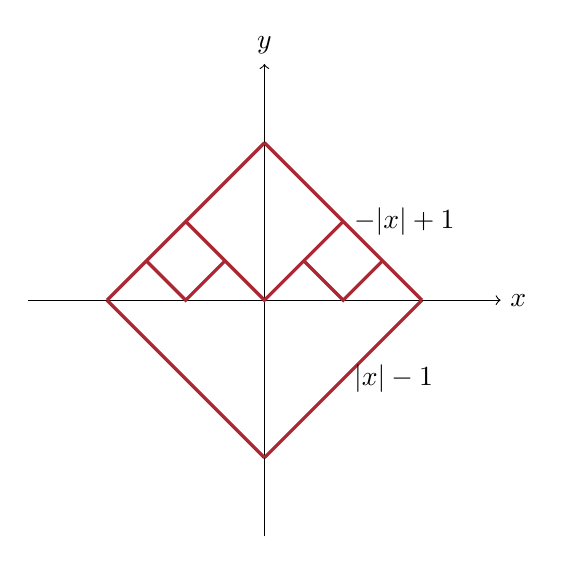
\begin{tikzpicture}[scale=2]

% Axis
      \draw[->] (-1.5,0.0) -- (1.5,0.0) node[anchor=west] {$x$};
      \draw[->] (0.0,-1.5) -- (0.0,1.5) node[anchor=south] {$y$};
% Radmacher Functions
    %k=0
      \begin{scope}[draw=Mahogany!80!Mulberry,line width=1.2pt]
        \draw (-1.0,0.0) -- (0.0,1.0);
        \draw (0.0,1.0)  -- (0.5,0.5) node[anchor=west] {$-|x|+1$} -- (1.0,0.0);

        \draw (-1.0,0.0)  -- (0.0,-1.0);
        \draw (0.0,-1.0)  -- (0.5,-0.5) node[anchor=west] {$|x|-1$} -- (1.0,0.0);
%k=1
        \draw (-0.5,0.5) -- (-0.0,0.0) -- (0.5,0.5);
%k=2
        \draw (-0.75,0.25) -- (-0.5,0.0) -- (-0.25,0.25);
        \draw (0.25,0.25) -- (0.5,0.0) -- (0.75,0.25);
      \end{scope}

    \end{tikzpicture}
  \end{center}
  \caption{Funzioni di \emph{Readmacher}. Soluzioni quasi ovunque dell'equazione einoidale.}
  \label{fig:cp2-01}
\end{figure}

Nel 1982 Crandal e Lions introdussero una differente nozione di soluzione debole (soluzioni viscose \cite[vedi][]{crand:lion}) per molte equazioni del primo e del secondo ordine, soddisfacente proprietà di esistenza, unicità e stabiltà. 
%%%%%%%%%%%%%%%%%%%%%%%%%%%%%%%%%%%%%%%%%%%%%%%%%%%%%%%%%%%%%%%%%%%%%%%%%%
%
%                            Section 2.2
%
%
%%%%%%%%%%%%%%%%%%%%%%%%%%%%%%%%%%%%%%%%%%%%%%%%%%%%%%%%%%%%%%%%%%%%%%%%%%
\section{Nozione di soluzioni viscose}
Inziamo col introdurre la definizione di soluzione viscosa per PDE del secondo ordine, cioè equazioni del tipo
\begin{equation}
\label{eq:cp2-02}
F(x,u,Du,D^2u) = 0\text{ con }F:\mathbb{R}^N\times\mathbb{R}\times\mathbb{R}^N\times S(N)\to \mathbb{R},
\end{equation}
con $S(N)$ insieme delle matrici simmetriche $N\times N$, $u$ una funzione a volori reali definita in un sottoinsieme $\mathcal{O}$ di $\mathbb{R}^N$ e $Du$,$D^2u$ corrispondono al gradiente ed alla matrice delle derivate seconde di $u$. Al fine di applicare la teoria a un equazione del tipo \eqref{eq:cp2-02} (\cite[][2]{crand:lion}), richiederemo che $F$ soddisfi le seguenti propietà
\begin{gather}
\label{eq:cp2-03}
F(x,r,p,X) \leq F(x,s,p,X) \quad \forall\,r\leq s,\\
\label{eq:cp2-04}
F(x,r,p,X) \leq F(x,r,p,Y) \quad \forall\,Y\leq X,
\end{gather}
con $r,s\in \mathbb{R},X,Y\in S(N)$ and $S(N)$ equipaggiato del solito ordine tra matrici. Se $F$ soddisfa \eqref{eq:cp2-03} allora si dirà \emph{ellitticamente degenere}, mentre se soddisfa \eqref{eq:cp2-04} si dirà \emph{propria}.

Da qui in avanti assumeremo sempre che $F$ soddisfi \eqref{eq:cp2-03}
e \eqref{eq:cp2-04} e che sia continua, a meno che non venga detto
diversamente. Prima di enunciare la definizione di soluzione di
viscosità, diamo una giustificazione euristica. Supponiamo che $u\in C^2$ su $\mathbb{R}^n$ e che
\[
F(x,u(x),Du(x),D^2u(x))\leq 0\, \forall x\in\mathbb{R}^n,
\]
cioè $u$ è una sottosoluzione classica di $F=0$. Supponiamo $\phi\in
C^2$ e $\hat{x}$ sia un massimo locale per $u-\phi$, dall'analisi
questo implica che $Du(\hat{x})=D\phi(\hat{x})$ e $D^2u(\hat{x})\leq
D^2\phi(\hat{x})$, quindi dalla \eqref{eq:cp2-03} segue
\[
F(x,u(\hat{x}),D\phi(\hat{x}),D^2\phi(\hat{x}))\leq F(x,u(x),Du(x),D^2u(x))\leq 0.
\]
Gli estremi di questa diseguaglianza non dipendono dalle derivate di $u$, quindi possiamo considerare un arbitraria funzione $u$ essere sotto soluzione di $F=0$ se
\begin{equation}
  \label{eq:cp2-01-add}
  F(x,u(\hat{x}),D\phi(\hat{x}),D^2\phi(\hat{x}))\leq 0
\end{equation}
ogniqualvolta $\phi\in C^2$ e $\hat{x}$ massimo locale di $u-\phi$.
Inoltre  per $x$ vicino a $\hat{x}$ è vero che $u(x)\leq u(\hat{x})-\phi(\hat{x}) + \phi(x)$, poichè $\phi\in C^2$ usando Taylor otteniamo
\begin{equation}
  \label{eq:cp2-05}
  u(x)\leq u(\hat{x})+\left<p,x-\hat{x}\right> + \frac{1}{2}\left<X(x-\hat{x}),x-\hat{x}\right> + o(|x-\hat{x}|^2)\,\, x\to\hat{x}
\end{equation}
con $p=D\phi(\hat{x})$ e $X=D^2\phi(\hat{x})$. Possiamo osservare che se la \eqref{eq:cp2-05} è soddisfatta per qualche $(p,X)\in\mathbb{R}^n\times S(N)$ e $u$ è due volte differenziabile, allora $p=Du(\hat{x})$ e $D^2u(\hat{x})\leq X$ (\emph{Osservazione} \ref{oss:cp2-01}). Quindi se $u$ è una soluzione classica per $F\leq 0$ segue che $F(x,u(x),p,X)\leq 0$ ogni qual volta è vera la \eqref{eq:cp2-05}. Ora possiamo dare la definizione di soluzione viscosa, che si basa proprio sulla \eqref{eq:cp2-05}
\begin{definizione}
\label{def:cp2-01}
Sia $F$ propria ed ellittica degenere e $\mathcal{O}\subset\mathbb{R}^n$.
Una sottosoluzione viscosa di $F=0$ su $\mathcal{O}$ è una funzione $u:\mathcal{O}\to\mathbb{R}$ continua tale che
\begin{equation}
  \label{eq:cp2-06}
  F(x,u(x),p,X)\leq 0\quad\forall x\in\mathcal{O}\text{ and }(p,X)\in J_{\mathcal{O}}^{2,+}u(x).
\end{equation}
Similmente, una sopra soluzione viscosa di $F=0$ su $\mathcal{O}$ è una funzione continua tale che
\begin{equation}
  \label{eq:cp2-07}
  F(x,u(x),p,X)\geq 0\quad\forall x\in\mathcal{O}\text{ and }(p,X)\in J_{\mathcal{O}}^{2,-}u(x).
\end{equation}
Infine, $u$ è una soluzione viscosa se è sia sotto che sopra soluzione.
\end{definizione}
Dove $J_{\mathcal{O}}^{2,+}u(x)$ rappresenta il \emph{superjet} del secondo ordine di $u$ nel puto $x$. Più precisamente sia $\mathcal{O}\subset\mathbb{R}^N$ arbitrario%
\footnote{Nelle dimostrazioni di esistenza, unicità e confronto viene preso localmento compatto \cite[vedi][10 §1]{crand:lion}.}
,  $u:\mathcal{O}\to\mathbb{R}$ e $\hat{x}\in\mathcal{O}$ allora
\[
J_{\mathcal{O}}^{2,+}u(\hat{x}) = \left\{(p,X)\in\mathbb{R}^n\times S(N):\,\text{ vale la \eqref{eq:cp2-05} per }\mathcal{O}\ni x\to\hat{x}\right\},
\]
quindi $J_{\mathcal{O}}^{2,+}u(x)$ definisce una mappa da $\mathcal{O}$ ad un sottoinsieme di $\mathbb{R}^n\times S(N)$. Una definizione simile si ottiene per il \emph{subjet} $J_{\mathcal{O}}^{2,-}u(x)$ basta invertire il segno della disuguaglianza.
\begin{osservazione}
Come si può notare dalla definizione, il ``superjet'' (lo stesso vale per il ``subjets'') dipende dall'insieme $\mathcal{O}$, tuttavia si può notare che il suo valore è lo stesso per tutti quegli insiemi $\mathcal{O}$ per i quali $x$ è un punto interno.  
\end{osservazione}

\begin{osservazione}
\label{oss:cp2-01}
Nella definizione di soluzione viscosa, la richiesta di continuità di $u$ può essere sostituita con quella di semicontinuà superiore(\emph{upper semicontinuos}) per le sotto soluzione e semicontinuà inferiore(\emph{lower semicontinuos}) per le sopra soluzione. Inoltre, notiamo che una funzione semicontinua sia superiormente che inferiormente è continua. Ricordiamo che  $u:L \to\mathbb{R}$ è
\begin{enumerate}
  \item \emph{upper semicontinuos} in $\hat{x}\in L$ se:
    \[
      \limsup_{x\downarrow\hat{x}}u(x)\leq u(\hat{x}).
    \]
  \item \emph{lower semicontinuos} in $\hat{x}\in L$ se:
    \[
      \liminf_{x\downarrow\hat{x}}u(x)\geq u(\hat{x}).
    \]
\end{enumerate}  

Seguendo la discussione fatta ad inizio sezione, se $u$ è una soluzione viscosa di $F\leq 0$, $\phi\in C^2$ in un intorno di $\mathcal{O}$ e $u-\phi$ ha un massimo locale in $\hat{x}\in\mathcal{O}$, allora è vera la \eqref{eq:cp2-01-add} ( stesso ragionamento per le sopra soluzioni). Questo motiva la richiesta per $u$ di essere semicontinua dall'alto (rispettivamente dal basso per le sopra soluzioni), in quanto è facile produrre massimi per funzioni semicontinue dall'alto.
Possiamo dire di più, la validità di \eqref{eq:cp2-01-add} per tutte le $\phi\in C^2$ tale che $u-\phi$ ha un massimo locale relativo ad $\mathcal{O}$, con $u$ semicontinua dall'alto, equivale a dire che $u$ è una sotto soluzione viscosa.  Infatti si può mostrare il seguente lemma (per maggiori dettagli \cite[vedi][§3]{giga:main})
\begin{lemma}
  \label{lem:cp2-01}
 Sia $\hat{x}\in\mathcal{O}$ localmente compatto%
\footnote{ Ricordiamo che un insieme di uno spazio metrico si dice localmente compatto se ogni punto ammette un intorno compatto.}
 e $u$ semicontinua dall'alto allora
\begin{enumi}
  \item  vale la seguente uguaglianza
\[
J_{\mathcal{O}}^{2,+}u(\hat{x}) = \left\{
\begin{aligned}
&(D\phi(\hat{x}),D^2\phi(\hat{x})):\\
\phi\in C^2&\text{ e $u-\phi$ ha massimo locale in $\hat{x}$}
\end{aligned}
\right\}
\]
  \item  In $(i)$ $\mathcal{O}$ può essere rimpiazzato da un intorno $\mathcal{O}'$ di $\hat{x}$ in $\mathcal{O}$.
\end{enumi}
\end{lemma}

\begin{proof}
Denotiamo con $J$ l'insieme a destra dell'uguaglianza in $(i)$ e poniamo $\hat{x}=0$ se così non fosse possiamo sempre traslare il tutto.
\begin{enumi}
\item  Prendiamo un elemento in $J$, allora $u-\phi$ ha massimo locale in $\hat{x}=0$ quindi
\[
\begin{aligned}
u(x) - u(0)\leq\phi(x) -\phi(0)&=\left<D\phi(0),x\right> + \frac{1}{2}\left<D^2\phi(0)x,x\right> +\\
+ o(|x|^2)\text{ per }x\to 0,
\end{aligned}
\]
avendo utilizzato un espansione di Taylor per $\phi$. Questo ci dice che $J_{\mathcal{O}}^{2,+}u(0)\supseteq J$.

Ora prendiamo $(p,X)\in J_{\mathcal{O}}^{2,+}u(0)$, cioè
\[
u(x) - u(0)\leq\left<p,x\right> + \frac{1}{2}\left<Xx,x\right> + \varepsilon(x),
\]
con $\varepsilon(x)/|x|^2\to 0$ per $x\to 0$.
Il problema è che $\varepsilon(x)$ non è detto che sia $C^2$. Poniamo 
\[
\omega_0(\sigma)=\sup\left\{\frac{|\varepsilon(x)|}{|x|^2}; |x|\leq\sigma,x\in\mathcal{O}\right\}
\]
così che $\omega_0$ è una funzione da $[0,\infty)$ in $[0,\infty)$ non decrescente e continua in $\sigma=0$ con $\omega_0(0)=0$, applicando un risultato noto \cite[vedi][§2 Lemma 2.1.9]{giga:main}, allora esiste una funzione $\theta\in C^2[0,\infty)$ tale che
\[
\begin{aligned}
&\omega_0(\sigma)|\sigma|^2\leq\theta(\sigma)\text{ per }\sigma\geq 0,\\
&\theta(0)=\theta'(0)=\theta''(0)=0,\,\theta'''(\sigma)\geq 0\text{ per }\sigma\geq 0.
\end{aligned}
\]
Poichè $|\varepsilon(x)|\leq\omega_0(|x|)|x|^2$, prendiamo una funzione $C^2$ del tipo
\[
\phi(x)=<p,x> + \frac{1}{2}<Xx,x> +\theta(|x|)
\]
così che $u-\phi$ ha massimo locale su $\mathcal{O}$ in $\hat{x}=0$ e $p=D\phi(0)$, $X=D^2\phi(0)$. Quindi $J_{\mathcal{O}}^{2,+}u(0)\subseteq J$.
\item  Segue dalla dimostrazione di $(i)$.
\end{enumi}
\end{proof}

\end{osservazione}

\begin{osservazione}
Si può facilmente verificare che se $u\in C^2$ è soluzione classica di \eqref{eq:cp2-02} ed $F$ è elliticamente degenere, allora $u$ è soluzione viscosa.
\end{osservazione}

\begin{esempio}
Riprendiamo l'equazione eiconale \eqref{eq:cp2-01} e mostriamo che la funzione $u(x) = -|x| + 1$ è una soluzione viscosa. Partiamo dall'osservare che questa funzione risolve classicamente l'equazione in $\mathbb{R}\setminus\{0\}$, quindi
calcoliamoci rapidamente il ``superjets'' e il ``subjets'' in $\hat{x}=0$
\[
\begin{aligned}
  J^{2,+}u(0) &= \left\{\left((-1,1)\times\mathbb{R}\right)\cup\left(\{-1,1\}\times [0,+\infty)\right)\right\}, \\
  J^{2,-}u(0) &= \left\{\emptyset\right\},
\end{aligned}
\]
applicando la definizione \ref{def:cp2-01} si osserva che $|p|\leq 1$ è vera per ogni $(p,X)\in J^{2,+}u(0)$, quindi è sotto soluzione e che $|p|\geq 1$ è banalmente verificata in quanto $J^{2,-}u(0)=\emptyset$. In conclusione $u(x)=-|x|+1$ e soluzione viscosa di \eqref{eq:cp2-01}.  
\end{esempio}

La definizione di soluzione viscosa qui presentata, può essere estesa anche al caso di equazioni paraboliche cioè del tipo
\begin{equation}
\label{eq:cp2-08}
u_t + F(t,x,u,Du,D^2u) = 0,
\end{equation}
dove ora $u=u(t,x)$ e $Du$, $D^2u$ stanno per $D_xu$ e $D^2_xu$. Per farlo dobbiamo ridefinire gli insiemi $J_{\mathcal{O}}^{2,\pm}$. Sia $\mathcal{O}\subset\mathbb{R}^N$, $T>0$ e $\mathcal{O}_T = (0,T)\times\mathcal{O}$, denotiamo con $\mathcal{P}_{\mathcal{O}}^{2,\pm}$ la variante parbolita dei ``superjets'' e ``subjets'' e andiamoli a definire; se $u:\mathcal{O}\to\mathbb{R}$ allora $\mathcal{P}_{\mathcal{O}}^{2,+}u(s,z)$ è costituito da $(a,p,X)\in\mathbb{R}\times\mathbb{R}^N\times S(N)$ se $(s,z)\in\mathcal{O}_T$ e
\[
\begin{aligned}
  u(t,x)\leq &u(s,z) +a(t-s)+\left<p,x-z\right>+\frac{1}{2}\left<X(x-z),x-z\right> \\
  &+o(|t-s|+|x-z|^2)\text{ per }\mathcal{O}_T\ni (t,x)\to(s,z),
\end{aligned}
\]
similarmente possiamo definire $\mathcal{P}_{\mathcal{O}}^{2,-}u(s,z)=-\mathcal{P}_{\mathcal{O}}^{2,+}(-u(s,z))$. Quindi in conclusione una sotto soluzione di \eqref{eq:cp2-08} su $\mathcal{O}_T$ è una funzione $u$ semicontinua dall'alto tale che
\[
a+F(t,x,u(t,x),p,X)\leq 0\text{ per }(t,x)\in\mathcal{O}_T,(a,p,X)\in\mathcal{P}_{\mathcal{O}}^{2,+}u(t,x),
\]
e una sopra soluzione una funzione semicontinua dal basso tale che
\[
a+F(t,x,u(t,x),p,X)\geq 0\text{ per }(t,x)\in\mathcal{O}_T,(a,p,X)\in\mathcal{P}_{\mathcal{O}}^{2,-}u(t,x),
\]
e quindi un soluzione viscosa se sono verificate entrambe le diseguaglianze.

\begin{osservazione}
Osserviamo che anche in questo caso $F$ soddisfa le proprietà \eqref{eq:cp2-03} e \eqref{eq:cp2-04}. Ed inoltre anche per i ``semijets'' parbolici vale un lemma del tipo \ref{lem:cp2-01} \cite[vedi][§3]{giga:main}.
\end{osservazione}

Le definizioni si posso estendere anche per $u$ ed $F$ arbitrarie, non necessariamente continue. Prima di vedere come, richiamiamo la definizione di inviluppo semicontinuo. Sia $h$ una funzione definita in $L\subset\mathbb{R}$ a valori in $\tilde{\mathbb{R}}=\mathbb{R}\cup\{\pm\infty\}$, definiamo inviluppo semicontinuo superiore $h^*$ e inferiore $h_*$ nel seguente modo
\begin{subequations}
\begin{align}
  \label{eq:cp2-03-1-add}%
  h^*(x) &= \lim_{r\downarrow 0}\sup_{\substack{|x-y|<r \\ y\in L}}h(y),\quad x\in\overline{L} \uptag{*} \\
  \label{eq:cp2-03-2-add}%
  h_*(x) &= \lim_{r\downarrow 0}\inf_{\substack{|x-y|<r \\ y\in L}}h(y),\quad x\in\overline{L} \subtag{*}
\end{align}
\end{subequations}
sono rispettivamente funzioni definite sulla chiusura di $L$ a valori in $\tilde{\mathbb{R}}$. In altre parole $h_*$ è la piu grande funzione semicontinua dal basso su $\overline{L}$ che è più piccola di $h$ su $L$, mentre $h^*$ è la più piccola funzione semicontinua dall'alto in $\overline{L}$ più grande di $h$ in $L$.
Prendiamo $\mathcal{O}\subset\mathbb{R}^N$ e consideriamo un sottoinsieme denso $W$ di $\Omega(\mathcal{O})=\mathcal{O}\times\mathbb{R}\times\mathbb{R}^N\times S(N)$ e sia $F=F(x,s,p,X):W\to\mathbb{R}$. Poichè $W$ è denso in $\Omega(\mathcal{O})$, gli inviluppi semicontinui $F_*$, $F^*$ sono definiti in $\Omega(\mathcal{O})$ con valori in $\tilde{\mathbb{R}}$.
\begin{definizione}
Una funzione $u:\mathcal{O}\to\mathbb{R}$ è chiamata una sotto soluzione viscosa (rispettivamente sopra soluzione) in $\mathcal{O}$ di \eqref{eq:cp2-02} se $u^*<\infty$ (resp. $u_*>-\infty$) in $\mathcal{O}$ e per ogni coppia $\phi\in C^2(\mathcal{O})$ e $\hat{x}\in\mathcal{O}$ soddisfacente $\max_{\mathcal{O}}(u^*-\phi)=(u^*-\phi)(\hat{x})$ (resp. $\min_{\mathcal{O}}(u_*-\phi)=(u_*-\phi)(\hat{x})$), vale che
\[
\begin{aligned}
&F_*(\hat{x},u^*(\hat{x}),D\phi(\hat{x}),D^2\phi(\hat{x}))\leq 0 \\
(\text{resp. }&F^*(\hat{x},u_*(\hat{x}),D\phi(\hat{x}),D^2\phi(\hat{x}))\geq 0)
\end{aligned}
\]
\end{definizione}
\begin{osservazione}
Applicando il lemma \ref{lem:cp2-01} possiamo dara una definizione generica di soluzione viscosa per l'equazione \eqref{eq:cp2-02} utilizzando i ``superjets'' e ``subjets''.
\end{osservazione}
Una definizione generica analoga vale anche nel caso di equazioni paraboliche del tipo \eqref{eq:cp2-08}.
\begin{definizione}
\label{def:cp2-02}
Una funzione $u:\mathcal{O}_T\to\mathbb{R}$ è chiamata una sotto soluzione viscosa (rispettivamente sopra soluzione) in $\mathcal{O}_T$ di \eqref{eq:cp2-08} se $u^*<\infty$ (resp. $u_*>-\infty$) in $\mathcal{O}_T$ e per ogni coppia $\phi\in C^2(\mathcal{O}_T)$ e $(\hat{x},\hat{t})\in\mathcal{O}_T$ soddisfacente $\max_{\mathcal{O}_T}(u^*-\phi)=(u^*-\phi)(\hat{x},\hat{t})$ (resp. $\min_{\mathcal{O}_T}(u_*-\phi)=(u_*-\phi)(\hat{x},\hat{t})$), vale che
\[
\begin{aligned}
&\phi_t(\hat{x},\hat{t}) + F_*(\hat{x},\hat{t},u^*(\hat{x},\hat{t}),D\phi(\hat{x},\hat{t}),D^2\phi(\hat{x},\hat{t}))\leq 0 \\
(\text{resp. }&\phi_t(\hat{x},\hat{t})+F^*(\hat{x},\hat{t},u_*(\hat{x},\hat{t}),D\phi(\hat{x},\hat{t}),D^2\phi(\hat{x},\hat{t}))\geq 0)
\end{aligned}
\]
\end{definizione}
\begin{osservazione}
In questo caso chiaramente $F$ è definita in $W_T$ denso in $\mathcal{O}_T\times\mathbb{R}\times\mathbb{R}^N\times S(N)$. E anche in questo caso possiamo dara una definizione che coinvolge i ``superjets'' e ``subjets'' parabolici, grazie ad una variante del lemma \ref{lem:cp2-01}. 
\end{osservazione}
Per risultati di esistenza, unicità e confronto sia per equazioni del tipo \eqref{eq:cp2-02} che \eqref{eq:cp2-08} \cite[vedi][]{crand:lion,giga:main,yun:giga}.
%%%%%%%%%%%%%%%%%%%%%%%%%%%%%%%%%%%%%%%%%%%%%%%%%%%%%%%%%%%%%%%%%%%%%%%%%%
%
%                            Section 2.3
%
%
%%%%%%%%%%%%%%%%%%%%%%%%%%%%%%%%%%%%%%%%%%%%%%%%%%%%%%%%%%%%%%%%%%%%%%%%%%
\section{Soluzioni viscose per il moto per curvatura media}
In questa sezione tratteremo equazioni paraboliche degeneri (cioè che verificano \eqref{eq:cp2-04}) del tipo
\begin{equation}
  \label{eq:cp2-09}
u_t + F(x,t,Du,D^2u) = 0
\end{equation}
in particolare nel caso in cui \eqref{eq:cp2-09} rappresenta un'equazione di evoluzione per superfici di livello di $u$.  Supporremo che $F$ sia geometrica cioè
\begin{equation}
  \label{eq:cp2-10}
F(x,t,\lambda p,\lambda X + \sigma p\otimes p) = \lambda F(x,t,p,X),\quad\lambda>0,\,\sigma\in\mathbb{R},
\end{equation}
per $p\in\mathbb{R}^N$ diverso da zero, $X\in S(N)$ e $\otimes$ denota il prodotto tensoriale in $\mathbb{R}^N$. Un tipico esempio di equazione che rientra in questo caso è
\[
u_t - |Du|\Div(\frac{Du}{|Du|}) = 0,
\]
l'equazione del moto per curvatura media. Iniziamo col vedere, tramite semplici conti, che questa verifica la condizione geometrica e di degenere ellitticità.
Come vedremo in dettaglio nella sezione successiva l'equazione per curvatura media si può riscrivere nel seguente modo
\[
u_t+F(Du,D^2u)=0,\quad\text{ con }F(p,X) = -\trace\left(\left(I-\frac{p}{|p|}\otimes\frac{p}{|p|}\right)X\right),
\]
con $I$ matrice identità $N\times N$.
Un semplice calcolo mostra che
\[
\begin{aligned}
F(\lambda p,\lambda X +\sigma p\otimes p)&=-\trace\left(\left(I-\frac{p}{|p|}\otimes\frac{p}{|p|}\right)\left(\lambda X+\sigma p\otimes p\right)\right)=\\
&=\lambda F(p,X)-\sigma\trace\left(\left(I-\frac{p}{|p|}\otimes\frac{p}{|p|}\right)p\otimes p\right).
\end{aligned}
\]
Poichè $(\overline{p}\otimes\overline{p})(p\otimes p)=p\otimes p$, con $\overline{p}=p/|p|$, la \eqref{eq:cp2-10} è banalmente verificata. Per dimostrare la condizione di degenere ellitticità basta mostrare che
\[
-\trace\left(\left(I-\frac{p}{|p|}\otimes\frac{p}{|p|}\right)\left(X-Y\right)\right)\leq 0\text{ con }X\geq Y.
\]
Osserviamo che la traccia del prodotto di due matrici definite non
negative è non negativo e poichè $X-Y\geq 0$,  basta mostrare che la matrice $B(p)= I-\overline{p}\otimes\overline{p}$, con $\overline{p}$ come sopra, è non negativa per $p\ne 0$, cioè che $\forall x\in\mathbb{R}^N$ $x^tB(p)x\geq 0$:
\[
x^tB(p)x=x^tx-x^t\frac{p}{|p|}\otimes\frac{p}{|p|}x=|x^2|-\frac{|p^tx|^2}{|p|^2}\geq |x|^2-\frac{|p|^2}{|x|^2}{|p|^2}=0
\]
nel penultimo passaggio abbiamo usato la disuguaglianza di Cauchy-Schwartz.

Risultati di esistenza, unicità e confronto sono stati dimostrati  per \eqref{eq:cp2-09} con
\begin{equation}
\label{eq:cp2-02-add}
u(0,x)=a(x)\in C_{\alpha}(\mathbb{R}),
\end{equation}
cioè $a(x)-\alpha$ è continua con supporto compatto in $\mathbb{R}^N$
ed $\alpha\in\mathbb{R}$ e per $F(x,t,p$\\$,X)$ ellitticamente degenere, geometrica, continua in $\mathbb{R}^N\times(0,T]\times(\mathbb{R}^N\setminus\{0\})\times S(N)$ e soddisfacente ulteriori due proprietà
\begin{subequations}
  \label{eq:cp2-12}
  \begin{align}  \label{eq:cp2-12-1}
    F_*(x,t,p,-I)&\leq c_{-}(|p|), \subtag{-}\\
     \label{eq:cp2-12-2} F^*(x,t,p,I)&\geq -c_{+}(|p|),  \subtag{+}
  \end{align}
\end{subequations}
per qualche $c_{\pm}(\sigma)\in C^1[0,\infty)$ e $c_{\pm}(\sigma)\geq c_0>0$ per qualche costante $c_0$. Iniziamo col notare che la $F$ del moto per curvatura media soddisfa le condizioni (\hyperref[eq:cp2-12-1]{\ref{eq:cp2-12}\ped{$\pm$}}); difatti $F(p,X)=-\trace\left(A(p)X\right)$ ed  essendo $F$ continua per $p\in\mathbb{R}^N\setminus\{0\}$ e geometrica  verifica le condizioni precedenti con
\[
c_{\pm}(\sigma)=\sup_{|p|=1}\trace\left(A(p)\right).
\]  
Per $p\ne 0$ abbiamo
\[
F_*(p,-I)=F(p,-I)=\trace\left(A(\overline{p})I\right)\leq\sup_{\overline{p}}\trace\left(A(\overline{p})\right)\text{ con }\overline{p}=p/|p|
\]
mentre per $p=0$, usando la definizione di inviluppo semicontinuo, otteniamo
\[
F_*(0,-I)=\inf_{|\overline{q}|=1}\trace\left(A(\overline{q})I\right)\leq\sup_{|\overline{q}|=1}\trace\left(A(\overline{q})\right),
\]
quindi soddisfa la \eqref{eq:cp2-12-1}; similmente si dimostra la \eqref{eq:cp2-12-2}.
\begin{osservazione}
Sotto le condizioni (\hyperref[eq:cp2-12-1]{\ref{eq:cp2-12}\ped{$\pm$}}), possiamo costruirci una sotto e sopra soluzione dell'equazione per il moto per curvatura media, per farlo basta applicare il seguente lemma
\begin{lemma}
Supponiamo $F$ geometrica e soddisfacente (\hyperref[eq:cp2-12-1]{\ref{eq:cp2-12}\ped{$\pm$}}) per qualche $c_{\pm}(\sigma)\in C^1[0,\infty)$ e $c_{\pm}(\sigma)\geq c_0>0$ per qualche costante $c_0$. Poniamo \[
u^{\pm}=\pm(t+\omega_{\pm}(\rho)),\quad \rho=|x|,\quad\omega_{\pm}(\rho)=\int_0^{\rho}\frac{\sigma}{c_{\pm}(\sigma)}d\sigma.
\]
Allora $u^-$ (resp. $u^+$) è una  sotto soluzione $C^2$ di \eqref{eq:cp2-09} in $\mathbb{R}\times\mathbb{R}^N$.
\end{lemma}
\begin{proof}
Dimostriamo il caso in cui $u^-$ è sotto soluzione se verifica la \eqref{eq:cp2-12-1}, l'altro è analogo. Per definizione di $u^-\in C^2(\mathbb{R}\times\mathbb{R}^N)$. Poichè $F_*$ è geometrica e
\[
\begin{aligned}
D&\omega_{-}(\rho)=\omega_{-}^{'}(\rho)D\rho \\
D^2\omega_{-}(\rho)&=\omega_{-}^{''}(\rho)D\rho\otimes D\rho+\omega_{-}^{'}(\rho)D^2\rho \\
&D^2\rho = \rho^{-1}(I-D\rho\otimes D\rho)
\end{aligned}
\]
dove l'ultima uguaglianza deriva dal fatto che $D\rho = D|x| = x/\rho$, quindi derivando giungiamo al risultato riportato sopra. Osservando che $\omega_{-}^{'}(\rho)> 0$ un semplice calcolo ci mostra che
\[
\begin{aligned}
F_*(x,t,Du,D^2u) &= F_{*}(x,t,-\omega_{-}^{'}(\rho)D\rho,-\omega_{-}^{'}(\rho)\rho^{-1}I+\sigma D\rho\otimes D\rho) \\
&=\omega_{-}^{'}(\rho)\rho^{-1}F_*(x,t,-\rho D\rho,-I),
\end{aligned}
\] 
con $\sigma = -(\omega^{''}(\rho)-\omega^{'}(\rho))$.
In conclusione abbiamo
\[
u_t + F_*(x,t,Du,D^2u) = -1 + \frac{1}{c_{-}(\rho)}F_*(x,t,-x,-I),
\]
in quanto  $\rho D\rho=x$, quindi per la \eqref{eq:cp2-12-1} otteniamo
\[
u_t + F_*(x,t,Du,D^2u)\leq 0
\]
e per la definizione \ref{def:cp2-02}, $u$ è sotto soluzione viscosa di \eqref{eq:cp2-09}.
\end{proof}
Applicando tale lemma con $c_{\pm}(\sigma)=\sup_{|\overline{p}|=1}\trace\left(A(\overline{p})\right)=N-1$ con $A(\overline{p})=I-\overline{p}\otimes\overline{p}$ otteniamo che
\[
u^{-}=-\left(t+\frac{|x|^2}{2(N-1)}\right).
\]
è una soluzione viscosa del moto per curvatura media, che rappresenta sfere che si contraggono. 
\end{osservazione}
Nel lavoro di Giga, Chen e Goto sono stati dimostrati teoremi di
esistenza, confronto e unicità per \eqref{eq:cp2-09} e dato iniziale
\eqref{eq:cp2-02-add}, noi qui riportiamo solo l'enunciato del
teoremi esistenza; per approfondimenti e dimostrazioni si veda \cite[][§4-6]{yun:giga}.
\begin{teorema}[Esistenza globale]
Sia $T>0$. Assumiamo che $F(t,p,X)$ sia continua in $(0,T]\times(\mathbb{R}^N\setminus\{0\})\times S(N)$, geometrica, ellitica degenere, soddisfacente le condizioni (\hyperref[eq:cp2-12-1]{\ref{eq:cp2-12}\ped{$\pm$}}) e tale che $ -\infty<F_*(t,0,O) = F^*(t,0,O)<\infty$, con  $O$ matrice $N\times N$ nulla. Allora per $a\in C_{\alpha}(\mathbb{R}^N)$ esiste una unica soluzione viscosa $u_a\in C_{\alpha}([0,T]\times\mathbb{R}^N)$ di \eqref{eq:cp2-09}-\eqref{eq:cp2-02-add} 
\end{teorema}
Per completare questa sezione, e per definire le soluzioni nel caso particolare del moto per curvatura media, vediamo come definire 
\[
F(p,X)=-\trace\left(\left(I-\overline{p}\otimes\overline{p}\right)X\right)
\]
in $p=0$, punto in cui è discontinua. In questo scenario c'è abbastanza arbitrarietà nello scegliere il valore di $F$, questo perchè come osservato da Crandal e Lions nell'analisi dell'equazione andiamo a porre $X=0$ quando $p=0$, quindi il valore in $p=0$ non importa purchè sia consistente  \cite[vedi][§9 p53]{crand:lion}.
\begin{enumi}
  \item Una prima possibilità è quella di calcolare esplicitamente gli inviluppi semicontinui $F_*$ e $F^*$ usando le definizione \eqref{eq:cp2-03-1-add} e \eqref{eq:cp2-03-2-add}, facciamo il conto per $F_*$
\[
F_*(0,X)=\lim_{r\downarrow 0}\inf_{\substack{|q|<r \\ q\in \mathbb{R}^N\setminus\{0\}}}F(q,X),
\]
ora $F(q,X)=-\trace\left(X\right)+\trace\left(\left(\overline{q}\otimes\overline{q}\right)X\right)$, con $\overline{q}=q/|q|$, quindi
\[
F_*(0,X)=-\trace\left(X\right)+\inf_{\substack{|\overline{q}|=1 \\ \overline{q}\in \mathbb{R}^N\setminus\{0\}}}\trace\left(\left(\overline{q}\otimes\overline{q}\right)X\right).
\]
Calcoliamoci il secondo addento dell'equazione precedente. Per farlo
ricordiamo che una matrice simmetrica a valori reali, come è $X$, è
diagonalizzabile con matrici ortonormali (Teorema spettrale) quindi
esiste $U$ tale che $UU^t=I$ e $X=U^t\Lambda U$, dove
$\Lambda=diag(\lambda_i(X))$, per ${\{i=1\dots n\}}$, con $\lambda_i$ autovalori di $X$. Applicando una propietà della traccia, ossia $\trace(AB)=\trace(BA)$, otteniamo che 
\[
\trace\left((\overline{q}\otimes\overline{q})X\right)=\trace\left((\overline{q}\otimes\overline{q})\Lambda\right)
\]
quindi
\[
\inf_{\substack{|\overline{q}|=1 \\ \overline{q}\in \mathbb{R}^N\setminus\{0\}}}\trace\left(\left(\overline{q}\otimes\overline{q}\right)X\right) = \inf_{\substack{|\overline{q}|=1 \\ \overline{q}\in \mathbb{R}^N\setminus\{0\}}}\sum_{i=1}^nq_i^2\lambda_i(X)
\]
con $q_i$ componenti del vettore $\overline{q}$. Il termine a destra dell'uguaglianza precednte è pari a $\lambda_{\text{min}}(X)$, mentre se ripetiamo il calcolo per $F^*$ nell'espressione precedente otterremo un $\sup\sum_{i=1}^nq_i^2\lambda_i(X)$ che è pari a $\lambda_{\text{max}}(X)$ (vedi \emph{osservazione} \ref{oss:cp2-02}).
Quindi $F^*$ e $F_*$ da usare nella definizione \ref{def:cp2-02} di soluzioni viscose per l'equazione del moto per curvatura media, sono
\begin{subequations}
\begin{align}
  \label{eq:cp2-13-1}%
  F_*(p,X) &=%
  \begin{cases}
   -\trace\left(\left(I-\overline{p}\otimes\overline{p}\right)X\right) &\text{ se } p\ne 0 \\
   -\trace\left(X\right)+\lambda_{\text{min}}(X) & \text{ se }p = 0
  \end{cases} \subtag{lse}\\
  \label{eq:cp2-13-2}%
  F^*(p,X) &=%
  \begin{cases}
   -\trace\left(\left(I-\overline{p}\otimes\overline{p}\right)X\right) &\text{ se } p\ne 0 \\
   -\trace\left(X\right)+\lambda_{\text{max}}(X) & \text{ se }p = 0
  \end{cases} \subtag{use}
\end{align}
\end{subequations}
\begin{osservazione}
  \label{oss:cp2-02}
  Proviamo che 
\[
\lambda_{\text{min}}(X)\leq\sum_{i=1}^nq_i^2\lambda_i(X)\leq\lambda_{\text{max}}(X),\quad |q| = 1,
\]
per induzione su $n$.
\begin{itemize}
  \item $N=1$, ovvia niente da dimostrare
  \item $N=2$, otteniamo che
\[
\sum_{i=1}^2q_i^2\lambda_i=\lambda_{\text{min}} + q_{\text{max}}^2(\lambda_{\text{max}}-\lambda_{\text{min}}),
\]
quindi essendo $q_{\text{max}}^2\leq 1$ il valore della somma precedente è sempre compresa tra il minimo ed il massimo dei valori $\lambda_{1,2}$ che ricordiamo essere numeri reali.
  \item $N=n$, supponiamo per semplicità che $\lambda_{\text{min}}=\lambda_1$
\[
\sum_{i=1}^nq_i^2\lambda_i=\lambda_1+\sum_{i=1}^{n-1}\hat{q}_i^2\hat{\lambda}_i,
\]
con $\hat{\lambda}_i=(\lambda_i-\lambda_1)>0$ e $\hat{q}=(q_2,\dots,q_n)$, $|\hat{q}|\leq 1$. Ora supponiamo, sempre per semplicità, $\hat{\lambda}_1$ il minimo dei $\hat{\lambda}_i$ e applicando l'ipotesi induttiva abbiamo
\begin{align}
0\leq\sum_{i=1}^{n-1}\hat{q}_i^2\hat{\lambda}_i(X)&=\hat{\lambda}_1|\hat{q}|+\sum_{i=2}^{n-1}\hat{q}_i^2(\hat{\lambda}_i-\hat{\lambda}_1) \notag\\
\hat{\lambda}_1|\hat{q}|+\sum_{i=2}^{n-1}\hat{q}_i^2(\hat{\lambda}_i-\hat{\lambda}_1)&\leq \hat{\lambda}_1+\sum_{i=2}^{n-1}\hat{q}_i^2(\hat{\lambda}_i-\hat{\lambda}_1)\leq\hat{\lambda}_{\text{max}}\notag \\
\intertext{e quindi}
\lambda_1=\lambda_{\text{min}}&\leq\sum_{i=1}^nq_i^2\lambda_i\leq\lambda_{\text{max}}\notag
\end{align}

\end{itemize}
\end{osservazione}
  \item Una altra definizione è quella proposta da Crandal e Lions \cite[vedi][§9]{crand:lion}
\begin{subequations}
\label{eq:cp2-14}
\begin{align}
  \label{eq:cp2-14-1}%
  \underline{F}(p,X) &=%
  \begin{cases}
   -\trace\left(\left(I-\overline{p}\otimes\overline{p}\right)X\right) &\text{ se } p\ne 0 \\
   -2||X|| & \text{ se }p = 0
  \end{cases} \subtag{cl_*}\\
  \label{eq:cp2-14-2}%
  \overline{F}(p,X) &=%
  \begin{cases}
   -\trace\left(\left(I-\overline{p}\otimes\overline{p}\right)X\right) &\text{ se } p\ne 0 \\
   +2||X|| & \text{ se }p = 0
  \end{cases} \subtag{cl^*}
\end{align}
\end{subequations}
Queste  sono  \eqref{eq:cp2-14-1} semicontinua inferiormente e
\eqref{eq:cp2-14-2} superiormente per $n=2,3$, \cite[vedi][§9]{crand:lion}.
\end{enumi}
\begin{osservazione}
Osserviamo che i teoremi sopra esposti valgono nel caso di moto per curvaura media, come abbiamo mostrato,  ed anche per la sua  generalizzazione cioè
\[
u_t -|Du|\Div\left(\frac{Du}{|Du|}\right) - \nu|Du| = 0,\quad\nu\in\mathbb{R},
\]
il cui flusso continua a verificare le ipotesi del teorema.
 Tuttavia possiamo estendere risultati di confronto ed esistenza, anche nel caso dell'equazione del moto per curvatura media che preserva il volume
\begin{equation}
  \label{eq:cp2-15}
  u_t(x,t)=|Du(x,t)|\Div{\left(\frac{Du(x,t)}{|Du(x,t)|}\right)}-\frac{\iint\Div{\left(\frac{Du(x,t)}{|Du(x,t)|}\right)}d\mu}{3V_0}x^tDu
\end{equation}
Sia $u:\Omega\times(0,T)\to\mathbb{R}$, una funzione level set di qualche superficie, allora l'integrale dell'equazione precedente lo possiamo riscrivere (vedi §\ref{cp:cp3-3})
\[
\mathcal{I}(u(x,t),t)=\frac{\int_{\Omega}-F(Du,D^2u)\delta(u(x,t))dx}{3V_0},
\]
Se tale termine ha una dipendenza locale da $u$ (come nel caso della
sfera in cui risulta essere costante vedi §\ref{cp:cp3-3}) allora la \eqref{eq:cp2-15} diventa
\[
u_t + F(Du,D^2u) + f(t,x,Du) = u_t +\tilde{F}(x,t,Du,D^2u)=0,
\]
con $F$ la stessa del moto per curvatura media e $f(x,t,Du)=\mathcal{I}(t)<x,Du>$.
Possiamo osservare che il flusso precedente rientra in 
\begin{equation}
\label{eq:cp2-16}
F(x,t,r,p,X) = F_0(t,r,p,X)+F_1(x,t,p),
\end{equation}
con $F_0$ soddisfacente le seguenti proprietà
\begin{enump}{f}
  \item $F_0:\overline{\Omega}\times[0,T]\times\mathbb{R}\times(\mathbb{R}^N\setminus{0})\times S(N)\to\mathbb{R}$ è continua
  \item $F_0$ ellittica degenere, cioè verifica la \eqref{eq:cp2-04}
  \item $ -\infty<F_*(x,t,0,O) = F^*(x,t,0,O)<\infty$
  \item Per qualche costante $c_0$ 
\[
      r\to F(x,t,r,p,X)+c_0r
\]
è una funzione non decrescente
\end{enump}
ed $F_1\in C(\overline{\Omega}\times[0,T]\times\mathbb{R}^N)$ tale che
\[
|F_1(x,t,p)-F_1(y,t,p)|\leq C(1+|p|)|x-y|,
\]
con qualche costante $C>0$ indipendente da $x$,
$y\in\overline{\Omega}$ e $p\in\mathbb{R}^N$. Sotto queste ipotesi,
risultati di confronto e esistenza vengono raggiunti da Crandal e
Lions, Giga e Goto, nel caso $\Omega$ limitato, per approfondimenti,
teoremi e dimostrazioni \cite[vedi][§3]{giga:main} e
\cite[][§8]{crand:lion}.
Nel caso di dipendenza non locale da $u$ in $\mathcal{I}(u,t)$, la
questione è ancora aperta e finora non sono stati raggiunti
risultati definitivi.
\end{osservazione}




\chapter{Costruzione ed analisi dello schema Semi-Lagrangiano}
In questo capitolo costruiremo ed analizzeremo uno schema Semi-Lagrangiano per l'equazione di curvatura media in $\mathbb{R}^3$.
Ricordiamo la nostra equazione :
\begin{equation}
\label{eq:cp3-01}
\begin{cases}
u_t = \Div\left(\frac{Du}{|Du|}\right)|Du|\quad (x_1,x_2,x_3)\in\mathbb{R}^3,t\in(0,T) \\
u(x,0) = u_0(x) \qquad \quad \mathbb{R}^3\times\{t = 0\}
\end{cases}
\end{equation}
con $Du$ il gradiente di $u$.
%%%%%%%%%%%%%%%%%%%%%%%%%%%%%%%%%%%%%%%%%%%%%%%%%%%%%%%%%%%%%%%%%%%%%%%%%%%%%
% Section 3.1 Costruzione dello schema
%
%%%%%%%%%%%%%%%%%%%%%%%%%%%%%%%%%%%%%%%%%%%%%%%%%%%%%%%%%%%%%%%%%%%%%%%%%%%%%%%%
\section{Costruzione dello schema MCM}

Partiamo dall'equazione \eqref{eq:cp3-01} e operiamo alcune manipolazioni algebriche, al fine di scrivere diversamente il termine del flusso. 
\begin{proposizione}
Vale la seguente serie di uguaglianze:
\[
\Div\left(\frac{Du}{|Du|}\right)|Du|=\trace\left(\left(I-\frac{DuDu^t}{|Du|^2}\right)D^2u\right)=\vec{v}_1^tD^2u\vec{v}_1+\vec{v}_2^tD^2u\vec{v}_2.
\]
con $\vec{v}_1$ e $\vec{v}_2$ autovettori della matrice $P=I-\frac{DuDu^t}{|Du|^2}$, definiti da :
\[
\vec{v_1}=
\begin{bmatrix}
\frac{-u_{x_3}}{\sqrt{u_{x_1}^2+u_{x_3}^2}} \\
0 \\
\frac{u_{x_1}}{\sqrt{u_{x_1}^2+u_{x_3}^2}}
\end{bmatrix}
\quad
\vec{v_2}=\frac{1}{|Du|}
\begin{bmatrix}
\frac{-u_{x_1}u_{x_2}}{\sqrt{u_{x_1}^2+u_{x_3}^2}} \\
\sqrt{u_{x_1}^2+u_{x_3}^2} \\
\frac{-u_{x_2}u_{x_3}}{\sqrt{u_{x_1}^2+u_{x_3}^2}}
\end{bmatrix}
\]
\end{proposizione}
\begin{proof}
Iniziamo con la prima uguaglianza, svolgendo esplicitamente $\Div\left(\frac{Du}{|Du|}\right)$ (senza riportare tutti i conti) otteniamo :
\[
|Du|\Div\left(\frac{Du}{|Du|}\right)=|Du|\left(\frac{\Div(Du)}{|Du|} -(Du)^tD^2u\frac{Du}{|Du|^3}\right) =
\]
\[
= \Delta u - \left<D^2u\frac{Du}{|Du|},\frac{Du}{|Du|}\right> .
\]
Ora ricordando che $\Delta u$ rappresenta il laplaciano della funzione $u$ e osservando che :
\[
\left<D^2u\frac{Du}{|Du|},\frac{Du}{|Du|}\right> = \left<\frac{1}{|Du|}(u_{x_1}(D^2u)^1+u_{x_2}(D^2u)^2+u_{x_3}(D^2u)^3),\frac{Du}{|Du|}\right> =
\]
\[
=\frac{1}{|Du|^2}(u_{x_1}<(D^2u)^1,Du>+u_{x_2}<(D^2u)^2,Du>+u_{x_3}<(D^2u)^3,Du> = 
\]
\[
=\trace\left(\frac{DuDu^t}{|Du|^2}D^2u\right),
\]
avendo indicato con $(D^2u)^n$ l'$n$-esima colonna della matrice delle derivate seconde della funzione $u$, giungiamo all'uguaglianza cercata:
\[
\Div\left(\frac{Du}{|Du|}\right)|Du| = \trace\left(\left(I-{\frac{DuDu^t}{|Du|^2}}\right)D^2u\right).
\] 
Ora occupiamoni della seconda uguaglianza. Iniziamo con il fare alcune osservazioni sulla matrice $P=I-\frac{DuDu^t}{|Du|^2}$. Questa è una matrice di proiezione, $3\times3$ a valori in $\mathbb{R}$, simmetrica ($P^t=P$) e idempotente ($P^2=P$), ammette due autovettori $\vec{v}_1$,$\vec{v}_2$ e vale la seguente decomposizione
\[
P=\sum_{i=1}^2\vec{v}_i\vec{v}_i^t=\sigma\sigma^t\quad\text{ con } \sigma=[\vec{v_1},\vec{v_2}],
\]
con $\sigma$ matrice $3\times2$ che ha come colonne gli autovettori di $P$. Detto ciò abbiamo: 
\[
\trace\left(\left(I-{\frac{DuDu^t}{|Du|^2}}\right)D^2u\right)=\trace\left(\sigma\sigma^tD^2\right)=\trace\left([\vec{v}_1,\vec{v}_2][\vec{v}_1,\vec{v}_2]^tD^2u\right)=
\]
\[
=\trace\left((\vec{v}_1\vec{v}_1^t+\vec{v}_2\vec{v}_2^t)D^2u\right)=\trace\left(\vec{v}_1\vec{v}_1^tD^2u\right)+\trace\left(\vec{v}_2\vec{v}_2^tD^2u\right)
\]
Ricordando i calcoli fatti nella dimostrazione della prima uguaglianza possiamo scrivere:
\[
\begin{split}
&\trace\left(\vec{v}_1\vec{v}_1^tD^2u\right)+\trace\left(\vec{v}_2\vec{v}_2^tD^2u\right)=\left<D^2u\vec{v}_1,\vec{v}_1\right>+\left<D^2u\vec{v}_2,\vec{v}_2\right>=\\
& =\vec{v}_1^tD^2u\vec{v}_1+\vec{v}_2^tD^2u\vec{v}_2.
\end{split}
\]
\end{proof}

Riformuliamo l'equazione \eqref{eq:cp3-01} nel seguente modo :
\begin{equation}
u_t=\vec{v}_1^tD^2u\vec{v}_1 + \vec{v}_2^tD^2u\vec{v}_2,
\end{equation}
e costruiamoci il metodo.
Approssimiano la derivata temporale con le differenze finite in avanti, mentre per il termine del flusso utilizziamo le derivate direzionali scegliendo come incremento $\sqrt{2\Delta t}$.
Quindi nel caso in cui $Du \ne 0$ e $u_{x_1}^2+u_{x_3}^2\ne 0$ otteniamo :
\[
\begin{split}
&\frac{u(x,t+\Delta t)-u(x,t)}{\Delta t} +O(\Delta t)= \frac{1}{4\Delta t}\bigl[u(x+\sqrt{2\Delta t}(\vec{v}_1+\vec{v}_2),t) +\\
& +u(x+\sqrt{2\Delta t}(-\vec{v}_1+\vec{v}_2),t) + u(x+\sqrt{2\Delta t}(\vec{v}_1-\vec{v}_2),t) \\
& + u(x+\sqrt{2\Delta t}(-\vec{v}_1-\vec{v}_2),t) - 4u(x,t)\bigr] + O(\Delta t)
\end{split}
\]
Osservando tale approssimazione, possiamo notare che i punti $(x + \sqrt{2\Delta t}(\pm\vec{v}_1 \pm\vec{v}_2))$ non necessariamente saranno i nodi della griglia, quindi è necessario introdurre un operatore di interpolazione $I[\cdot]$.
Per completare la costruzione consideriamo una griglia spaziale $x_j=(j_1\Delta x,j_2\Delta x,j_3\Delta x)$ con $j=(j_1,j_2,j_3)$ multi-indice in $\mathbb{Z}^3$ ed una griglia temporale $t^n=n\Delta t$ con $n\in\mathbb{N}$.
Indichiamo con $u_j^n$ l'approssimazione di $u$ nel punto della griglia $(x_j,t^n)$ e con $D_j^n$ l'approssimazione del gradiente di $u$ nel suddetto punto. Quindi il nostro schema semi-lagrangiano risulta :
\begin{equation}
\label{eq:cp3-02}
u_j^{n+1} = \frac{1}{4}\sum_{+,-}I[u^n](x_j+\sqrt{2\Delta t}(\pm\vec{v}_1\pm\vec{v}_2)).
\end{equation} 
\begin{osservazione}
Questa costruzione non è applicabile nel caso in cui 
\begin{equation}
\label{eq:cp3-01-add}
Du = 0 \text{ o } u_{x_1}^2+u_{x_3}^2 = 0. 
\end{equation}
Quindi per distinguere i due casi dal punto di vista numerico, introduciamo una soglia $s$ ed una costante $C$. In modo tale che il verificarsi del caso \eqref{eq:cp3-01-add} è rappresentato numericamente dalle disequazioni
\[
|D_j^n|\le C\Delta x^s\text{ e }|(D_j^n)_1^2+(D_j^n)_3^2|\le C\Delta x^s.
\]
\end{osservazione}
Nel caso in cui siamo sotto la soglia, possiamo procedere in due modi diversi.
\begin{enumerate}
  \item Approssimiamo la nostra soluzione nel punto $(x_j,t^{n+1})$, con la media dei primi vicini:
    \begin{equation}
      \label{eq:cp3-03-add}
      u_j^{n+1}=\frac{1}{6}\sum_{i\in\delta(j)}u_i^n,
    \end{equation}
dove $\delta(j)=\left\{(j_1\pm 1,j_2,j_3),(j_1,j_2\pm 1,j_3),(j_1,j_2,j_3\pm 1)\right\}$. Questa rappresentazione, non è altro che un'approssimazione dell'equazione del calore $u_t=\Delta u$ in $\mathbb{R}^3\times(0,T)$. Difatti usando Eulero in avanti per la derivata temporale e differenze finite centrate per quella spaziale abbiamo:
\[
\begin{aligned}
  \frac{u_j^{n+1}-u_j^n}{\Delta t}=\varepsilon&\frac{u_{j_1 + 1,j_2,j_3}^n +
    u_{j_1 - 1,j_2,j_3}^n + u_{j_1,j_2 + 1,j_3}^n + u_{j_1,j_2 - 1,j_3}^n}{\Delta x^2} + \\
    &+ \frac{u_{j_1,j_2,j_3 + 1}^n + u_{j_1,j_2,j_3 - 1}^n - 6u_j^n}{\Delta x^2},
\end{aligned}
\]
scegliendo $\varepsilon=\frac{\Delta x^2}{6\Delta t}$ otteniamo la \eqref{eq:cp3-03-add}.
Tale scelta è giustificata dal fatto che, come vedremo nella sezione successiva, il moto per curvature media è consistente con l'approssimazione dell'equazione del calore a patto di adottare, come soluzione viscosa, la definizione (riferimento formula) proposta da \emph{Crandall} in **ref.

  \item Utilizziamo l'approssimazione dell'equazione $u_t=\frac{1}{2}\Delta u$:
    \begin{equation}
      \label{eq:cp-04-add}
      u_j^{n+1}=u_j^n +\frac{1}{2}\frac{\Delta t}{\Delta x^2}\left(6u_j^n - \sum_{i\in\delta(j)}u_i^n\right).
    \end{equation}
Tale scelta è giustificata, in quanto il moto per curvatura media risulta essere consistente con l'equazione $u_t=\frac{1}{2}\Delta u$, (vedi sezione successiva) prendendo come soluzione viscosa la definizione standard (riferimento formula) presente in **rif. L'unico problema è che la \eqref{eq:cp-04-add}
richiede una CFL parabolica, che non è presente nel nostro schema essendo \emph{semi-lagrangiano}; un modo per aggirare il problema è quello di usare uno schema implicito nell'approssimazione di  $u_t=\frac{1}{2}\Delta u$.
\end{enumerate}
Scegliendo, ad esempio, la prima alternativa il nostro schema MCM completo diventa:
\begin{equation}
  \label{eq:mcm-schema}
  u_j^{n+1}=
  \left\{
  \begin{aligned}
    &   &\scriptstyle|D_j^n|>&\scriptstyle C\Delta x^s\\ 
    &\frac{1}{4}\sum_{+,-}I[u^n](x_j+\sqrt{2\Delta t}(\pm\vec{v}_1\pm\vec{v}_2)),  &\scriptstyle\mathbf{and} \\
    &  &\scriptstyle|(D_j^n)_1^2+(D_j^n)_3^2|&\scriptstyle >C\Delta x^2 \\
    &  &  \\
    &  &\scriptstyle|D_j^n|\leq&\scriptstyle C\Delta x^s \\
     & \frac{1}{6}\sum_{i\in\delta(j)}u_i^n,   &\scriptstyle\mathbf{and} \\
  &  &\scriptstyle|(D_j^n)_1^2+(D_j^n)_3^2| &\scriptstyle\leq C\Delta x^s.
  \end{aligned}   
  \right.
\end{equation}

%%%%%%%%%%%%%%%%%%%%%%%%%%%%%%%%%%%%%%%%%%%%%%%%%%%%%%%%%%%%%%%%%%%%%%%%%%%%%%
% Section 3.2 Consistenza dello schema
%
%%%%%%%%%%%%%%%%%%%%%%%%%%%%%%%%%%%%%%%%%%%%%%%%%%%%%%%%%%%%%%%%%%%%%%%%%%%%%%
\section{Consistenza dello schema}
Occupiamoci ora dell'analisi della consitenza dello schema. Prima di tutto ricordiamo che , per un dato schema numerico $S(x_j,u_j^n,Du_j^n)$ , l'errore di troncamento locale (o LTE) $\tau_j^n$ è l'errore che si genera pretendendo che la soluzione esatta soddisfi lo schema numerico :
\[
\tau_j^n=\frac{u(x_j,t^{n+1})-S(x_j,u(x_j,t^n),Du(x_j,t^n))}{\Delta t}
\]
Si definisce anche errore di troncamento totale la quantità
\[
\tau(\Delta t,\Delta x) := \max_{j,n} |\tau_j^n|.
\]
In generale un metodo si dirà consistente quando il suo LTE è infinitesimo rispetto all'incremento. Mentre si dirà consitente di ordine $p$ in tempo e $q$ in spazio se :
\[
\tau(\Delta t,\Delta x) = O(\Delta t^p +\Delta x^q).
\] 
Nel nostro caso, in quanto l'equazione che approssimiamo è singolare quando il gradiente  $Du$ si annulla oppure quando $u_{x_1}^2+u_{x_3}^2=0$, è necessario introdurre una definizione di consistenza più generale.
\begin{definizione}
Sia $(\Delta x_m,\Delta t_m)$ una seguenza generica di parametri di discretizzazione e sia $(x_{j_m},t^{n_m})\in G\times\left\{0,\dots,\Delta t_mN\right\}$ una seguenza generica di nodi, tale che per $m\to\infty$,
\[
(\Delta x_m,\Delta t_m)\to0 \quad\text{ e } (x_{j_m},t^{n_m})\to(x,t).
\]
E sia inoltre $\phi\in C^{\infty}(\mathbb{R}^3\times(0,t])$ e $\phi^{n_m-1}\equiv(\phi(x_{j_m},t^{n_m-1})_{x_{j_m}}$. Allora lo schema $S$ è detto consistente se
\begin{equation}
\label{eq:cp3-03}
\begin{split}
&\phi_t(x,t)+\underline{F}(D\phi(x,t),D^2\phi(x,t))\le \\
&\le\liminf_{m\to\infty}\frac{\phi(x_{j_m},t^{n_m})-S(x_{j_m},\phi_{j_m}^{n_m-1},D\phi_{j_m}^{n_m-1})}{\Delta t_m}\le \\
&\le\limsup_{m\to\infty}\frac{\phi(x_{j_m},t^{n_m})-S(x_{j_m},\phi_{j_m}^{n_m-1},D\phi_{j_m}^{n_m-1})}{\Delta t_m}\le \\
&\le\phi_t(x,t)+\overline{F}(D\phi(x,t),D^2\phi(x,t)).
\end{split}
\end{equation}
\end{definizione}
\begin{osservazione}
Osserviamo che se $F$ è continua allora il $\limsup$ ed il $\liminf$ nell'espressione \eqref{eq:cp3-03} coincidono, quindi la definizione si riduce a quella classica di consistenza.
\end{osservazione}

Indichiamo con $u(x,t)$ una soluzione regolare di \eqref{eq:cp3-01} e con $u(x_j,t^n)$ il suo valore sui nodi della griglia.
Prima di procedere con la consistenza, facciamo le seguenti ipotesi sull'errore commesso nell'approssimazione del gradiente e nell'interpolazione:
\begin{gather}
\label{eq:cp3-04}
||I[u^n](\cdot)-u(\cdot,t^n)||_{\infty}\le C_1\Delta x^r\quad\forall n\in\mathbb{N} \\
\label{eq:cp3-05}
|D_j[u^n]-Du(x_j,t^n)|\le C_2\Delta x^q\quad\forall n\in\mathbb{N}\quad\forall x_j, 
\end{gather}
con $C_1$ e $C_2$ costanti positive che dipendono così come gli ordini $r$ e $q$ dal metodo scelto per l'interpolazione e per l'approssimazioni del gradiente. Nel nostro caso abbiamo scelto entrambi i metodi di ordine $2$, quindi $r=q=2$.

%%%%%%%%%%%%%%%%%%%%%%%%%%%%%%%%%%%%%%%%%%%%%%%%%%%%%%%%%%%%%%%%%%%%%%%%%%%%%%
% SubSection 3.2.1 Caso DU != 0
%
%%%%%%%%%%%%%%%%%%%%%%%%%%%%%%%%%%%%%%%%%%%%%%%%%%%%%%%%%%%%%%%%%%%%%%%%%%%%%%
\subsection{Caso $Du \ne 0$}

Consideriamo il caso in cui $Du(x,t)\ne 0$ e $u_{x_1}(x,t)^2+u_{x_3}(x,t)^2\ne 0$, vista la regolarità di $u$, esiste un intorno di $(x,t)$ in cui le due espressioni precedenti si mantengono vere, quindi almeno asintoticamente:
\[
|D_j^n|\ge C\Delta x^s\text{ e }|(D_j^n)_1^2+((D_j^n)_3^2|\ge C\Delta x^s
\]
per cui possiamo applicare lo schema nella forma \eqref{eq:cp3-02}.

Abbiamo definito $\sigma=[\vec{v}_1,\vec{v}_2]^t$ quindi ponendo  $\vec{b}=[\pm1,\pm1]^t$ possiamo riscrivere il termine generico della sommatoria in \eqref{eq:cp3-02} come
\[
I[u^n](x_j+\sigma(D_j^n)\sqrt{2\Delta t}\vec{b}).
\]
Ora calcolando lo jacobiano di $\sigma$ per un qualsiasi vettore $p$ in $\mathbb{R}^3$ (senza riportare tutto il conto) si dimostra che:
\[
\left|J_{\sigma}(p)\right|^2=\frac{1}{p_1^2+p_3^2},
\]
dove come norma è stata scelta quella di Frobenius. Quindi applicando $\sigma[\cdot]$ al gradiente e sfruttando il fatto che $(D_j^n)_1^2+(D_j^n)_3^2\ge C\Delta x^s$, possiamo concludere che la funzione $\sigma$ risulta lipschitziana con costante $L_{\sigma}\le\frac{1}{C\Delta x^s}$.
Inoltre, avendo preso la $u$ sufficientemente regolare, anche essa sarà lipschitiziana con costatne $L_u$ e con $|Du|< M$. Assumiamo anche che $|u_{tt}(x,t)|\le C$ in modo tale da limitare l'errore di troncamento per l'approssimazione temporale.
 Analizziamo il prima addendo della sommatoria nell'espressione \eqref{eq:cp3-02} e facciamo alcune manipolazioni algebriche
\begin{equation}
\label{eq:cp3-06}
\begin{split}
& I[u^n](x_j+\sigma(D_j^n)\sqrt{2\Delta t}\vec{b}) = I[u^n](x_j+\sigma(D_j^n)\sqrt{2\Delta t}\vec{b}) - \\
& +u(x_j+\sigma(D_j^n)\sqrt{2\Delta t}\vec{b},t^n) + u(x_j+\sigma(D_j^n)\sqrt{2\Delta t}\vec{b},t^n)- \\
& + u(x_j+\sigma(Du(x_j,t^n))\sqrt{2\Delta t}\vec{b},t^n)+ u(x_j+\sigma(Du(x_j,t^n))\sqrt{2\Delta t}\vec{b},t^n).
\end{split}
\end{equation}
Stimiamo la parte destra di \eqref{eq:cp3-06}. Per la prima differenza applichiamo la stima dell'errore di interpolazione quindi
\begin{equation}
  \label{eq:cp3-07}
  \begin{split}
    |I[u^n](x_j+\sigma(D_j^n)\sqrt{2\Delta t}\vec{b}) &- u(x_j+\sigma(D_j^n)\sqrt{2\Delta t}\vec{b},t^n)|\le \\
    & \le C_1\Delta x^r,
\end{split}
\end{equation}
mentre per la seconda utilizzando la lipschitianità di $u$ , di $\sigma$ e la stima dell'errore di aprrossimazione del gradiente ottendo:
\begin{equation}
  \label{eq:cp3-08}
  \begin{split}
    |u(x_j+\sigma(D_j^n)\sqrt{2\Delta t}\vec{b},t^n) &- u(x_j+\sigma(Du(x_j,t^n))\sqrt{2\Delta t}\vec{b},t^n)|\le \\
    & \le M\sqrt{2\Delta t}\frac{C_2}{C}\Delta x^{q-s}.
  \end{split}
\end{equation}
Usando \eqref{eq:cp3-07} e \eqref{eq:cp3-08} in \eqref{eq:cp3-06} otteniamo
\[
\begin{split}
&I[u^n](x_j+\sigma(D_j^n)\sqrt{2\Delta t}\vec{b})=u(x_j+\sigma(Du(x_j,t^n))\sqrt{2\Delta t}\vec{b},t^n)+O(\Delta x^r)+ \\
& +O(\Delta x^{q-s}\sqrt{2\Delta t}).
\end{split}
\]
Sviluppiamo ora $u(x_j+\sigma(Du(x_j,t^n))\sqrt{2\Delta t}\vec{b},t^n)$ con una serie di Taylor del terzo ordine in un intorno del punto $x_j$:
\begin{equation}
\label{eq:cp3-09}
\begin{split}
&u(x_j+\sigma(Du(x_j,t^n))\sqrt{2\Delta t}\vec{b},t^n) = u(x_j,t^n)+ \\
&+\left<Du(x_j,t^n),\sigma(Du(x_j,t^n))\vec{b}\right>\sqrt{2\Delta t} +\\
&+\left<D^2u(x_j,t^n)\sigma(Du(x_j,t^n))\vec{b},\sigma(Du(x_j,t^n))\vec{b}\right>\Delta t + \\
&+T_3(\Delta t^{\frac{3}{2}}\sigma(Du(x_j,t^n))\vec{b},D^3u(x_j,t^n))+O(\Delta t^2), 
\end{split}
\end{equation}
non abbiamo esplicitato i termini del terzo ordine in quanto , mettondo tutto insieme, si eliminano cosi come i termini del primo ordine data la simmetria dei $4$ punti $x_j+\sigma(Du(x_j,t^n))\vec{b}\sqrt{2\Delta t}$ con $b=[\pm 1,\pm 1]^t$. Alla fine otteniamo che:
\begin{equation}
\label{eq:cp3-010}
\begin{split}
& S(x_j,u(x_j,t^n),Du(x_j,t^n)) = \\
& = u(x_j,t^n) + \vec{v}_1^tD^2u(x_j,t^n)\vec{v}_1 + \vec{v}_2^tD^2u(x_j,t^n)\vec{v}_2 + \\
& + O(\Delta x^r) + O(\Delta x^{q-s}\Delta t^{\frac{1}{2}}) + O(\Delta t^2).
\end{split}
\end{equation}
Ora sviluppando  anche il termine $u(x_j,t^{n+1})$ e applicando la definizione generale di consistenza \eqref{eq:cp3-03} otteniamo 
\[
\begin{split}
&\frac{u(x_j,t^{n+1})-S(x_j,u(x_j,t^n),Du(x_j,t^n))}{\Delta t}= u_t(x_j,t^n) + \\
&  -\vec{v}_1^tD^2u(x_j,t^n)\vec{v}_1 -\vec{v}_2^tD^2u(x_j,t^n)\vec{v}_2 + \\
& +O(\frac{\Delta x^r}{\Delta t}) + O(\frac{\Delta x^{q-s}}{\Delta t^{\frac{1}{2}}}) + O(\Delta t)
\end{split}
\]
questa per $(\Delta t,\Delta x)\to O$ e $(x_j,t^n)\to(x,t)$ risulta soddisfatta, nella forma classica, se $\Delta x = o(\Delta t^{\frac{1}{r}})$ e $\Delta x^{q-s}=o(\Delta t^{\frac{1}{2}})$

\end{document}
